\section{Method}

The goal of this thesis was to gauge the fault tolerance of approximate computing tools using fault injection. The faults in question were injected in software for practical reasons as hardware fault injection requires significantly more effort, and in LLVM-IR in an effort to make the results independent of language.

The tools that were tested were floatsmith and \taffo{}.

Prerequisite to testing the tools is installing the tools. \taffo{} depends on LLVM 14 or 15 to run, and is at the time of writing not compatible with newer versions of LLVM (the most recent version is 20). To install LLVM 15 you can build it from the source code following the instructions found at llvm.org. On certain GNU/linux distributions you may also install llvm through your package manager (if supported by the LLVM organization), but you may need to add the LLVM repository  to your package manager for this to work. 

Building \taffo{} was only successful when using pre-built binaries. 
The other tool that was used was floatsmith. This can be installed the easiest using their provided docker image, and mounting the project you want to perform experiments on.

\subsection{Bitwise fault injection}
Bitwise fault injection was done thorugh manually performing an XOR operation in LLVM IR on the values to be subjected to faults. Table~\ref{table:xor_truth_table} shows the truth table for two bit inputs through an XOR-gate. The output is 1 if and only if either input A or input B is 1 while the other is 0. If using input B as a bit mask of which bits to flip, we can see in the table that the output becomes the opposite of input A for all cases of input B being 1, and when input B is 0 all outputs are the same as input A. Such an operation on two 8-bit numbers is shown in figure~\ref{fig:xor_operation}. The output of the XOR operation shows that the output is the same as the input, except for the bit that is marked with red, which has been flipped.

\begin{table}[htb]
    \centering
\caption{Truth table for XOR function}
    \label{table:xor_truth_table}
\begin{tabular}{c|c|c}\label{table:xor_truth_table}
     input A& input B& XOR output \\
     0&0&0\\
     1&0&1\\
     0&1&1\\
     1&1&0
\end{tabular}
    
\end{table}



\begin{figure}[h!]
    \centering
    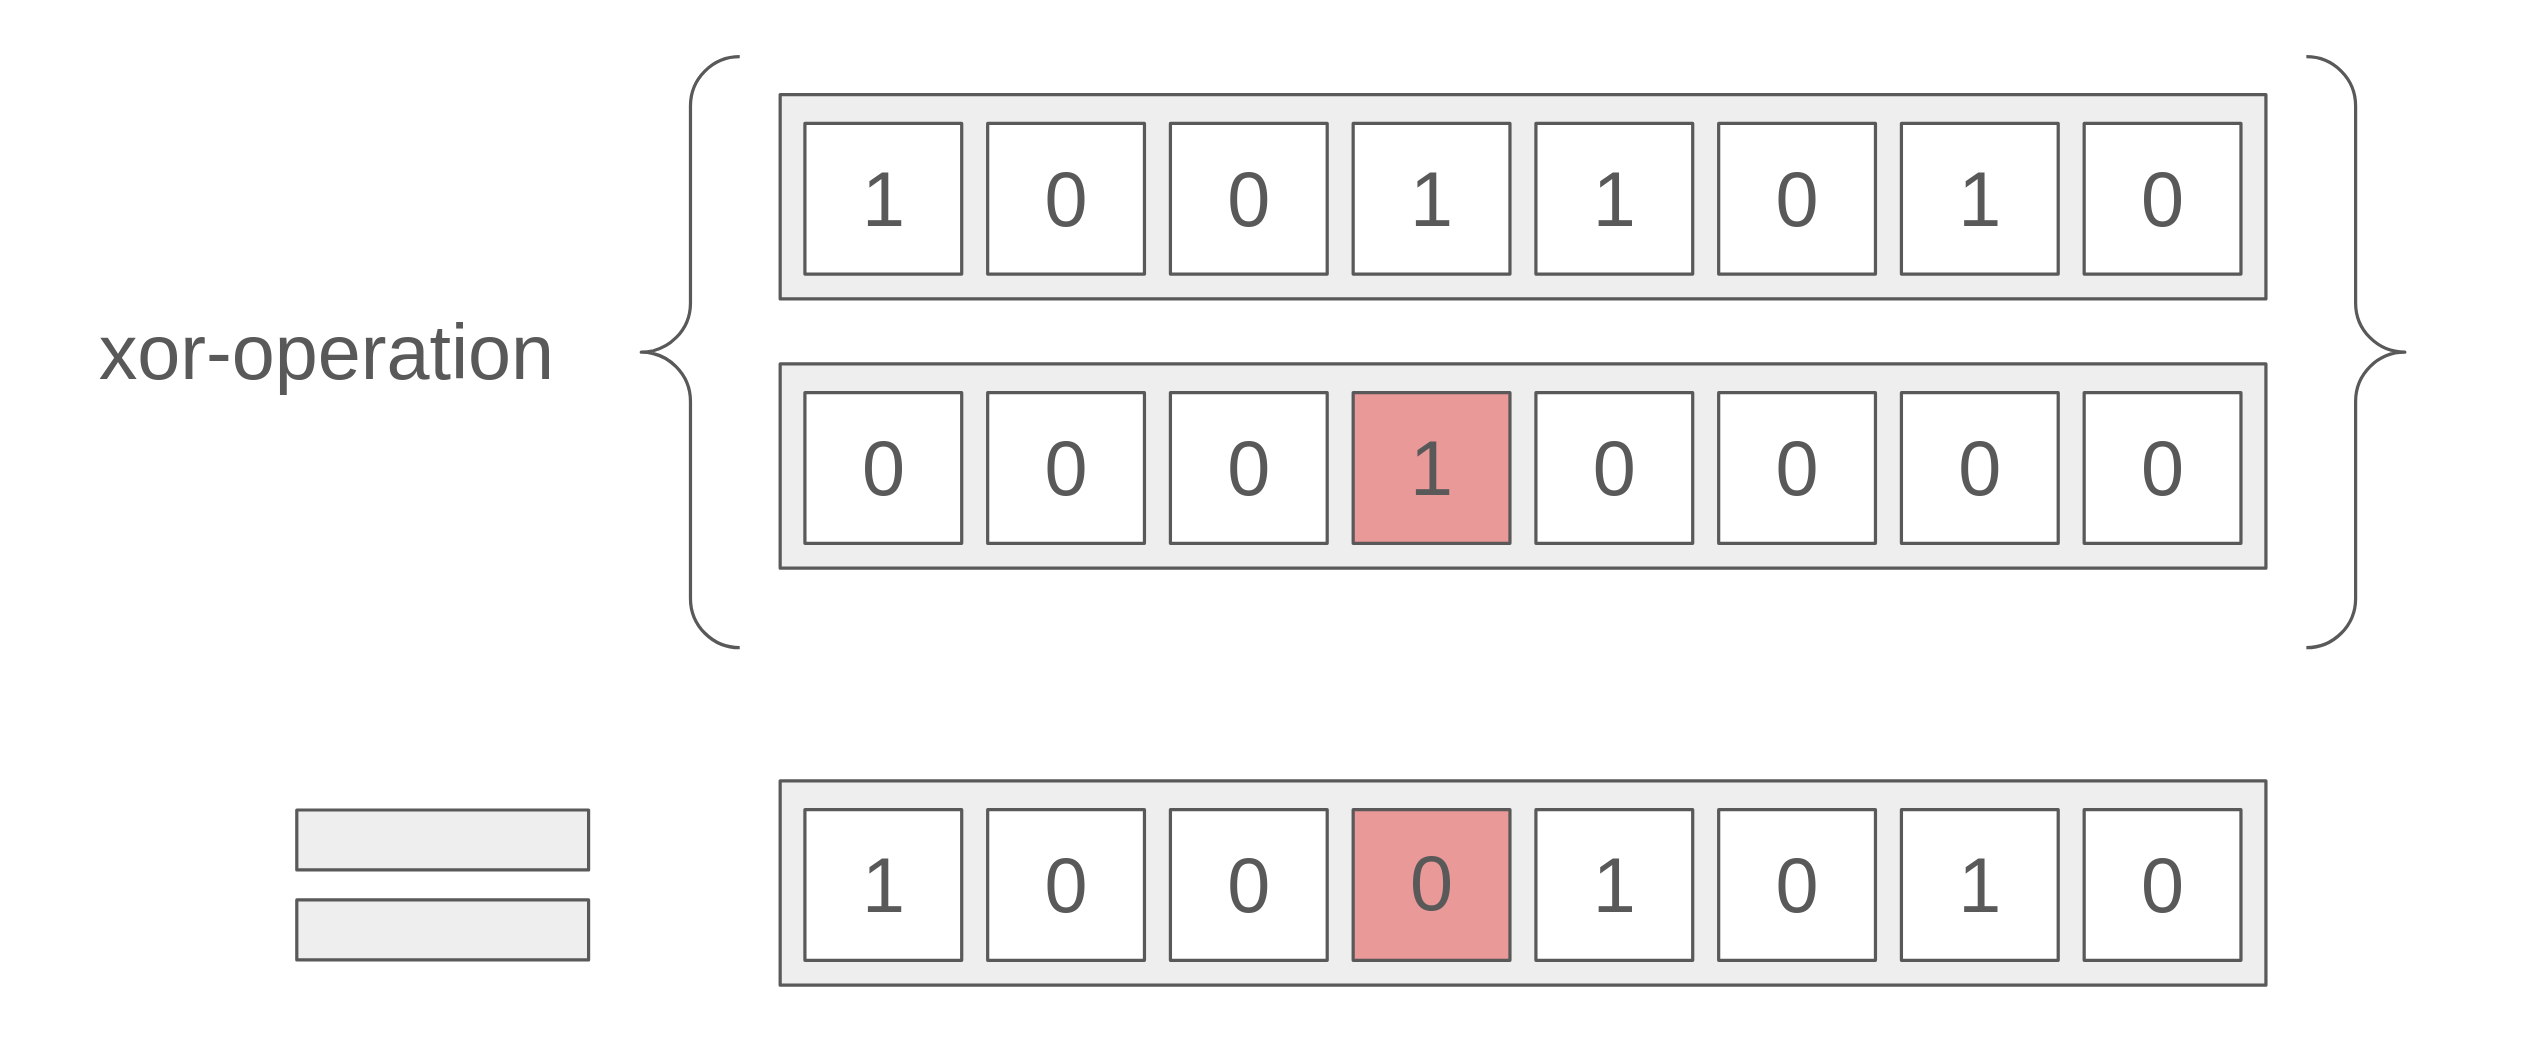
\includegraphics[width=0.5\linewidth]{Images/xor_operation.png}
    \caption{An example XOR operation between two numbers.}
    \label{fig:xor_operation}
\end{figure}

This was applied directly in LLVM-IR using LLVM-IR commands to perform a bit flip on a data variable within the running code. Code listing~\ref{listing:llvm_ir_fixed} shows how the bit flip was implemented for the fixed point implementation, and listing~\ref{listing:llvm_ir_float} shows the bitflip for the floating point implementation.



The result of the division is selected as the value to perform fault injection on, as there are only two division operations in both programs which makes the likelihood of the location being equivalent in both the floating point and fixed point IR files significant.
Two temporary variables, \%temp1 and \%temp2, are introduced, where \%temp1 is a 64 bit integer with value 1 shifted left however many bits necessary to inject a bit in the desired location. Listing~\ref{listing:llvm_ir_fixed} injects a bit in bit index number 4, making the last 8 bits of \%temp1 look like the mask number (with the bit highlighted in red) shown in figure~\ref{fig:xor_operation}.
The variable \%temp2 stores the result of the XOR operation between the result of the division in \%18 and the bit mask from \%temp1, and is then placed where \%18 ordinarily would be in the variable \%s10\_22fixp4.

\begin{lstlisting}[caption=fixed point bit flip in llvm-ir, label=listing:llvm_ir_fixed]

  %18 = sdiv i64 %16, %17, !taffo.info !109
  %temp1 = shl i64 1, 4
  %temp2 = xor i64 %temp1, %18
  %s10_22fixp4 = trunc i64 %temp2 to i32, !taffo.info !110
\end{lstlisting} 

\begin{lstlisting}[caption=floating point bit flip in llvm-ir, label=listing:llvm_ir_float]
  %temp1 = fdiv double %24, %26
  %temp2 = shl i64 1, 4
  %temp3 = bitcast double %temp1 to i64
  %temp4 = xor i64 %temp2, %temp3
  %27 = bitcast i64 %temp4 to double
\end{lstlisting}

Flipping a bit in the floating point implementation requires first performing a bitcast operation on the floating point number to be fault injected, \%temp1 in listing~\ref{listing:llvm_ir_float}. This means simply marking the bits in the memory location of \%temp1 as an integer, without actually changing any of the bits. This has to be done because the number 1 stored as a fixed point number is all zeros except the least significant bit which is 1, and a floating point binary representation contains several bits set to 1 in the exponent part of the number due to the exponent offset, see~\ref{section:approximate_computing_through_reducing_bits}. After the fault injection is performed, the fault injected variable then needs to be bitcast back to a floating point number.

The first fault injection campaign consisted of single bit fault injections. This consisted of taking a sample benchmark from the \taffo{} repository, compiling it to an intermediate format, in this case the LLVM IR, then flipping single bits one location at a time, and building it to a fault injected executable. For \taffo{}, which converts floating point values to lower precision fixed point values, this requires creating a fault injected version for both the fixed and floating point intermediate format.

For each pair of fault injected executables, the outputs are compared between each other and the original floating point implementation.

To streamline injections, a helper script was created based on the existing scripts in the \taffo{} repository. This allows a user to compile the selected benchmark from a list of benchmarks to LLVM IR, inject faults in a user-selected location in the code, then change the bit location of this fault, and compile many different versions of the same benchmark with different faults injected in the same location. The script then runs all the benchmarks and collects output. Finally a python script that reads these outputs collects and compares them in a human readable format.

The scripts are rather ad-hoc and requires some editing of code depending on the amount of bits that the user of the scripts wants to flip for one location.

The comparison script written in python was written in a separate repository with tests, and simply copied over. This process would have benefited from some kind of streamlining as well. 

\section{AI use}
AI was for the most part not used in neither the report nor the project part of the thesis, save for one instance. During a period of very slow progression, there was an attempt to coerce chatGPT to make sense of the build errors given by \taffo{} when trying to build it using clang15 built from source in debug mode. This led to many answers, though unfortunately no good ones. This only served to reinforce my opinion that relying on large language models for anything is a net waste of time. 
